\section{Proposal}

\subsection{This Proposal}
Simulating the Milky Way and M31 merger event opens a unique opportunity to study galaxy formation. Because of the vast amount of information we can obtain from the galaxies, it is the most accurate simulation achievable for merger events, allowing incredibly in-depth analysis of the characteristics of elliptical galaxies, galaxy formation, and the evolution of the universe. 

In this project, I will test $\Lambda$CDM theory by comparing Hernquist, NFW, and Einasto halo density profiles with simulated results using the GADGET-3 N-body simulation of the Milky Way and M31 merger. After determining the profile with the best fit, I will compare the remnant's dark matter velocity curve with the model's expected velocity curve to determine if the Milky Way and M31 remnant suffers from the cusp-core problem of $\Lambda$CDM cosmology.

\subsection{Methods}
The Milky Way and M31 merger remnant is theorized to be a large elliptical galaxy \cite{vanderMarel2012}. The density profiles of large elliptical galaxy halos can be fit to an NFW profile (as described by \cite{Navarro1997}) outlined in Equation \textbf{\ref{NFW profile}}. Here, $\rho_{dm}$ is the characteristic density and $r_{dm}$ is the characteristic radius. An example of a NFW density profile can be seen in \textbf{Figure \ref{NFW prof graph}}.

\smallskip
\begin{equation}
    \rho(r) = \rho_{dm} \left( \frac{r}{r_{dm}} \right)^{-1} \left(1 + \frac{r}{r_{dm}} \right)^{-2} 
    \label{NFW profile}
\end{equation}
\smallskip

After small, systematic deviations in the NFW profiles became apparent, the Einasto profile provided extra pliability for improved fitting. The Einasto density profile, first used by \cite{Einasto1965} to fit stars to the Milky Way, has been adopted by \cite{Navarroetal2004} to describe the density profile of dark matter halos. The Einasto profile is given by Equation \textbf{\ref{Einasto profile}}, where $r_{-2}$ is the radius where $ -\frac{d\log(\rho)}{d\log(r)}=-2$ and $\rho_{-2} = \rho(r_{-2})$. The parameter $\alpha$ has been found to increase with halo mass for redshifts of $z=0$ \cite{Frenk2012}.

\begin{equation}
    \rho(r) = \rho_{-2}\exp \left( \left( \frac{-2}{\alpha} \right) \left( \left( \frac{r}{r_{-2}} \right)^{\alpha} -1\right)\right)
    \label{Einasto profile}
\end{equation}
\smallskip

The Hernquist density profile was derived from the spherical galaxy density profile from \cite{Jaffe1983}. This was done to resemble the $R^{\frac{1}{4}}$ law at small radii \cite{Hernquist1990}. Hernquist density profile given by Equation \textbf{\ref{Hernquist profile}}, where $a$ is a scale length.

\begin{equation}
    \rho(r) = \frac{M_{halo}}{2\pi} \frac{a}{r(r+a)^{3}}
    \label{Hernquist profile}
\end{equation}
\smallskip

For proper analysis, I want to take the \textit{equilibrium} density profiles of the remnant, so I will analyze the final high resolution snap number (801) of the \textit{halo} component for the merged Milky Way and M31 galaxies.

After fitting each density profile to the remnant's DM halo density profile via scipy optimize curve fitting, I will perform a least squared test to determine which profile provides the best fit for the halo remnant. Each profile has a corresponding velocity curve; however, for simplicity, I will determine the adequate velocity profile equation once a density profile has been established. 

\begin{wrapfigure}{hR}{0.5\textwidth}
  \begin{center}
    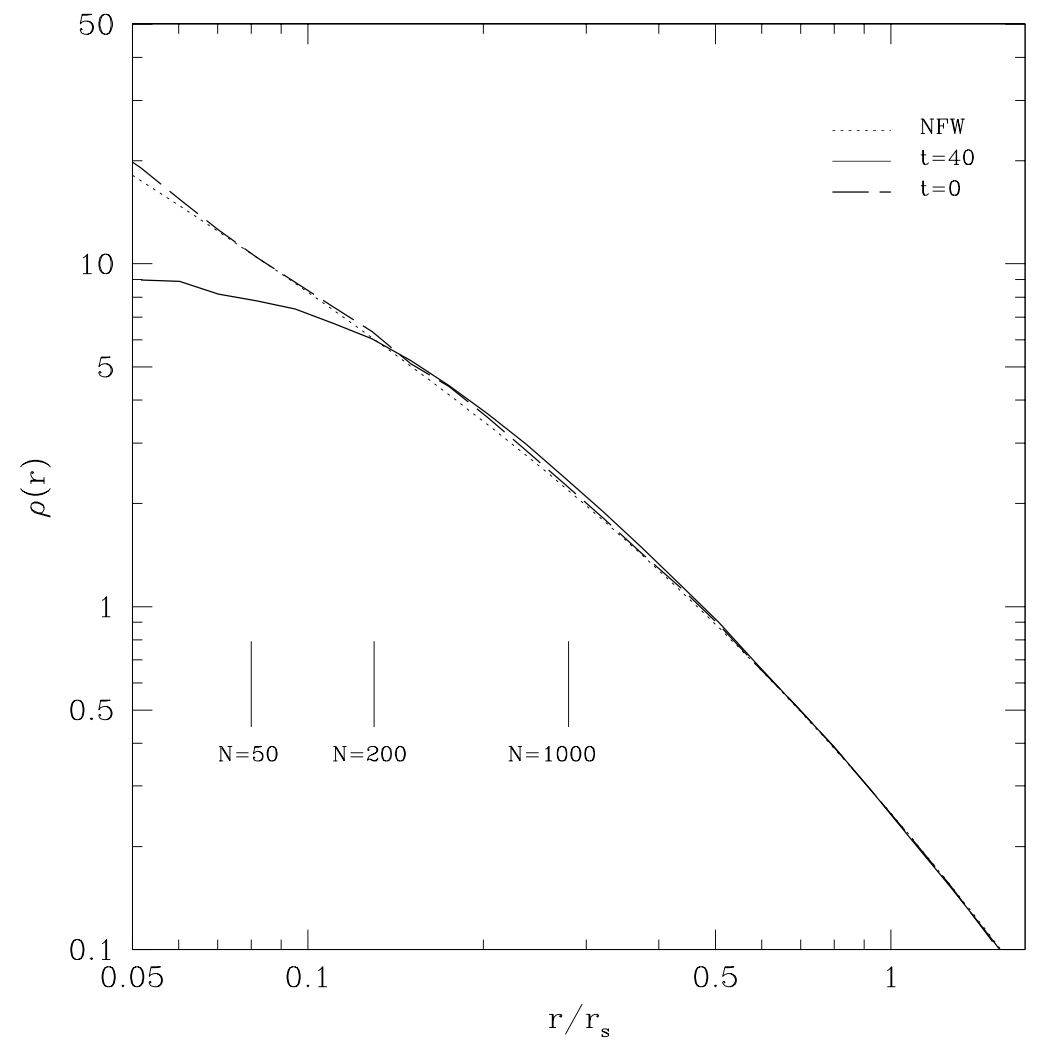
\includegraphics[width=0.48\textwidth]{Figures/NFWdensprof.png}
  \end{center}
  \caption{Example of NFW density profile from \cite{Prada2013}. Here, $r_{s}$ is scale radius.}
  \label{NFW prof graph}
\end{wrapfigure}

Lastly, I will overlay the expected and simulated velocity curves to identify if there is a significant difference between the two profiles. If the percent difference between the two profiles is $ <5\% $ on average, I will conclude that the Milky Way and M31 merger does not violate $\Lambda$CDM cosmology via the cusp-core problem. 

%

%\vspace{\baselineskip}
%\vspace{\baselineskip}
%\vspace{\baselineskip}
\subsection{Hypothesis}
The GADGET-3 simulation is an N-body, smoothed, hydrodynamical simulation that represents the initial dark matter halo of each galaxy in a Hernquist profile \cite{vanderMarel2012}. It is uncertain if a Hernquist profile will be the most accurate fit for the halo remnant. However, due to the profile's vital role in initializing the simulation, I hypothesize that it will be the best fit after the merger has occurred and equilibrium is reached. Due to the size of the merged DM halo remnant, I also expect that the theoretical and simulated velocity profiles will have no significant difference and therefore will not violate $\Lambda$CDM theory.